\documentclass[oneside,10pt,letterpaper]{book}

\usepackage{formato_cdt}          % El rollo de la CDT
\newcommand{\Titulo}{Manual de usuario: encargado}
\usepackage{formato_propio}       % Nuestro rollo
\usepackage{manual_de_usuario}

\begin{document}
\maketitle
\frontmatter
\tableofcontents
\mainmatter
%%=========================================================
\chapter{Uso General Del Sistema}
\section{Entorno De Trabajo}
En esta sección se describe el entorno de trabajo del sistema, se explica la disposición
de los elementos principales y comunes de las pantallas, los colores, la iconografía, componentes, etc.
utilizados dentro del sistema y el uso general del sistema.

\subsection{Diseño}
	\UMDesignFigure{inicio_Solicitante}{Inicio de Solicitante}
Se puede observar en la parte superior, en el encabezado de la página,
el menú del solicitante donde éste puede regresar a la pantalla de inicio,
salir o configurar su cuenta. En esta opción se puede cambiar la contraseña
y el correo si se desea.

Más abajo, encontramos el perfil del usuario, donde se mostrará el nombre
del mismo. 

Para hacer las reservaciones y otras funciones, todo se mostrará en la zona
de trabajo.


\subsection{Iconografía}
	En el sistema se utilizan iconos para denotar las diferentes operaciones que el usuario puede realizar
en el sistema. Los iconos utilizados se describen a continuación:
Nota: Desarrollo tiene que tener sus íconos para que el equipo de plantillas pueda generar el comando específico
\begin{Iconography}
	\item \ICexample Icono de Ejemplo
	\item \ICCancel  Permite cancelar un proceso en el momento que el usuario lo desee.
	\item \ICConfirm Permite confirmar los datos ingresados por el usuario.
	\item \ICQuery	 Permite generar y consultar estadísticas con base en los préstamos efectuados.
	\item \ICUnlockA Icono principal de inicio de sesión
	\item \ICEmail	Hace referencia al campo de correo electrónico
	\item \ICManageLoan  Accede a la gestión de préstamos
	\item \ICManageResource Accede a la gestión de recursos
	\item \ICTime	Hace referencia a los horarios disponibles de reservación
	\item \ICHome	Realiza una referencia a la pagina de inicio o home
    \item \ICName	Denota el campo o apartado de texto
	\item \ICPassword	Denota el campo o apartado de password
	\item \ICBooking Hace referencia a un calendario, donde se podrá seleccionar una fecha
	\item \ICStudyRoom  Hace referencia a una sala de estudio.
	\item \ICExpRoom  Hace referencia a una sala de exposiciones.
	\item \ICWorkRoom Hace referencia a una sala de trabajo
	\item \ICLogOut	Permite cerrar la sesión del usuario en cuestión.
	\item \ICUser   Hace referencia a la cuenta del usuario.
\end{Iconography}
\subsection{Organización}
	Las funcionalidades del sistema se encuentran organizadas por
un menú que se localiza en la parte lateral izquierda, el 
cual contiene lo siguiente:

\begin{enumerate}
	\item Inicio
	\item Gestionar usuarios
	\item Gestionar préstamos
	\item Consultar estadísiticas
	\item Salir
\end{enumerate} 


\subsection{Componentes Utilizados}
	En esta sección se explican los diferentes componentes que se utilizan para capturar o mostrar
información en el sistema.
\OComponent{Componente de Ejemplo}{example}{Componente de ejemplo}
Se describe el componente.

%% Manual de usuario
%% Departamento de Apoyo Técnico.
%% Índice de los procesos contenidos.

\chapter{Proceso Iniciar Sesión}
	Este capítulo explica el proceso que se lleva a cabo para ingresar al 
	sistema con un identificador y una contraseña. 
	Se tiene la siguiente interfaz:
	
%	\begin{figure}[hbtp]
%		\centering
%		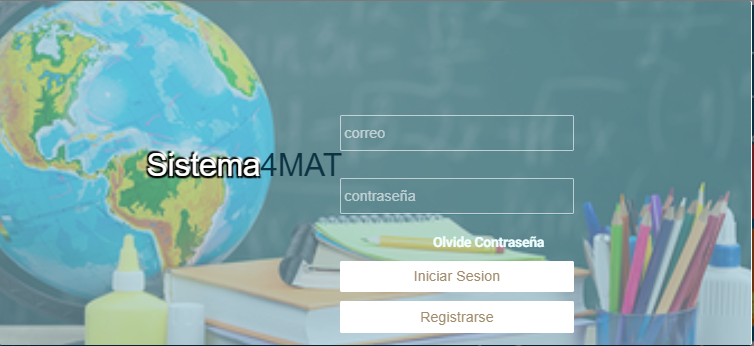
\includegraphics[scale=0.3]{images/Interfaz/IUGS00_login.png}
%		\caption{Iniciar sesión}
%	\end{figure}

%%\section{Información general de Iniciar sesión}
%%	\subsection{Información del usuario}

\subsection{Información de los préstamos}

\subsection{Información de la encuesta}


\section{Paso 1. Iniciar sesión}
	Se ingresan los datos de identificación para iniciar una sesión.
\subsection{Subpaso 1-A: Ingresar credenciales}
\begin{itemize}
	\item Ingrese identificador.
	\item Ingrese contraseña.
	\item Presione el botón \textbf{Entrar}. Este paso puede derivar
		en los errores \textbf{Error E1-A}, \textbf{Error E1-B} y 
		\textbf{Error E1-C}.
\end{itemize}
Observación 1: un identificador está compuesto por diez dígitos.

\subsection{Error E1-A: usuario no registrado}
El identificador que se ingresó no se encuentra registrado en el sistema,
debe dirigirse al Departamento de Apoyo Técnico para registrarlo.
\begin{itemize}
	\item Presionar \textbf{Aceptar} en la ventana emergente 
		\textbf{IUGS-30: usuario no registrado}
\end{itemize}

\subsection{Error E1-B: contraseña equivocada}
La contraseña que ingresó no concuerda con el valor que se tiene almacenado.
\begin{itemize}
	\item Presionar \textbf{Aceptar} en la ventana emergente 
		\textbf{IUGS-31: contraseña equivocada}
\end{itemize}

\subsection{Error E1-C: solicitante sancionado}
Usted ha sido sancionado por el Departamento de Apoyo Técnico.
\begin{itemize}
	\item Presionar \textbf{Aceptar} en la ventana emergente 
		\textbf{IUGS-32: solicitante sancionado}
\end{itemize}
	\subsection{Bienvenida del administrador de 4MAT}

Se muestra la interfaz de bienvenida.
	\begin{figure}[hbtp]
		\centering
		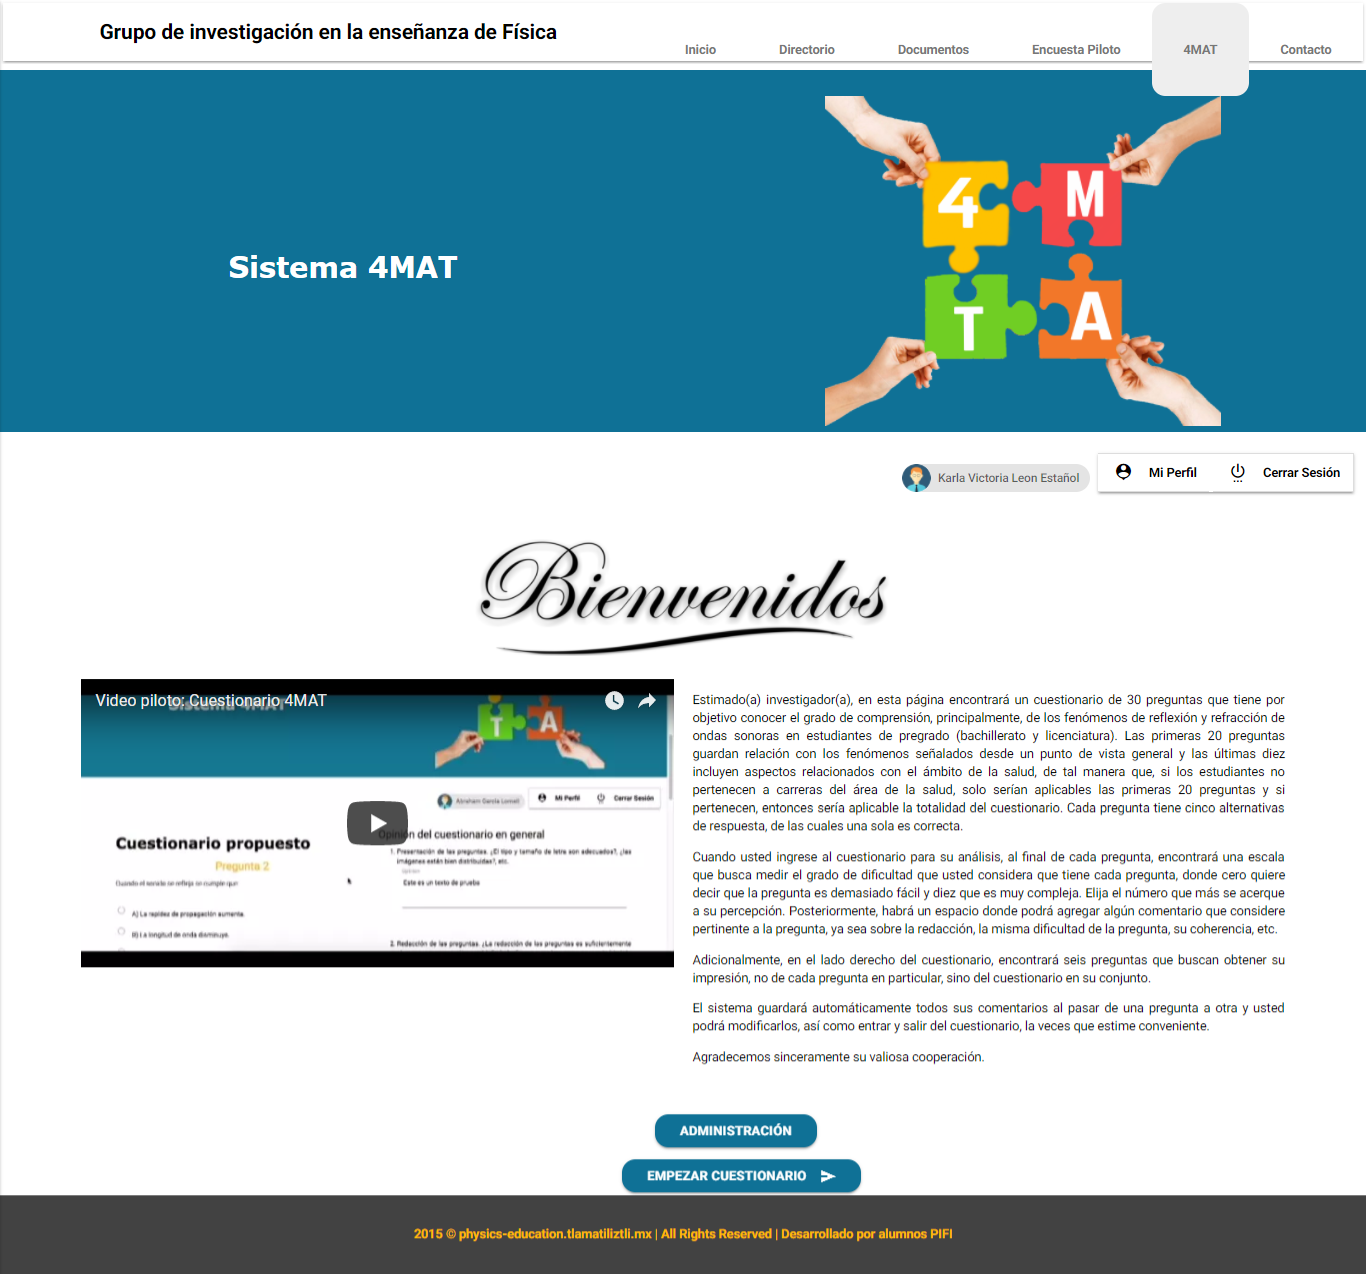
\includegraphics[scale=0.3]{images/Interfaz/IUGS01_binevenida.png}
		\caption{Bienvenida para Administrador}
	\end{figure}
	
La cual contiene los siguientes elementos:
	\begin{itemize}
		\item Menú para las demás secciones de la pagina
			\begin{figure}[hbtp]
		
			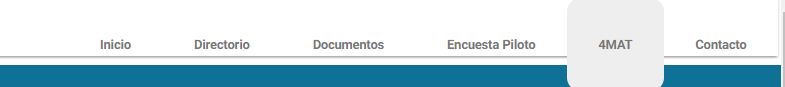
\includegraphics[scale=0.6]{images/Interfaz/IUGS01_menu.png}
			\caption{Menú}
		\end{figure}
		\item Menú de administración de usuario.
			\begin{figure}[hbtp]
		
			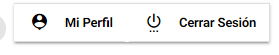
\includegraphics[scale=0.6]{images/Interfaz/IUGS01_menuadmin.png}
			\caption{Menú para datos personales}
		\end{figure}
		
		\item Vídeo explicando como usar la pagina web
		 \begin{figure}[hbtp]
		
			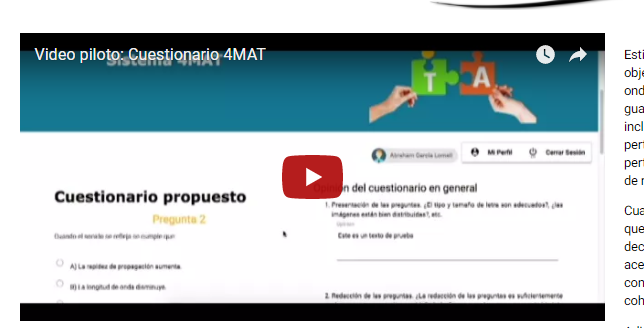
\includegraphics[scale=0.6]{images/Interfaz/IUGS01_video.png}
			\caption{Vídeo explicativo}
		\end{figure}
		\item Botón de administración para consultar estadísticas.
			 \begin{figure}[hbtp]
		
			
\includegraphics[scale=0.6]{images/Interfaz/IUGS01_botonadmin.png}
			\caption{Botón de administración}
		\end{figure}
		\item Botón de iniciar cuestionario. Donde nos presentará el
		cuestionario que se aplicó a los maestros y estudiantes.
		
		
	\end{itemize}
	
	
\chapter{Proceso Iniciar Sesión}
	Este capítulo explica el proceso que se lleva a cabo para ingresar al 
	sistema con un identificador y una contraseña. 
	Se tiene la siguiente interfaz:
	
	\begin{figure}[hbtp]
		\centering
		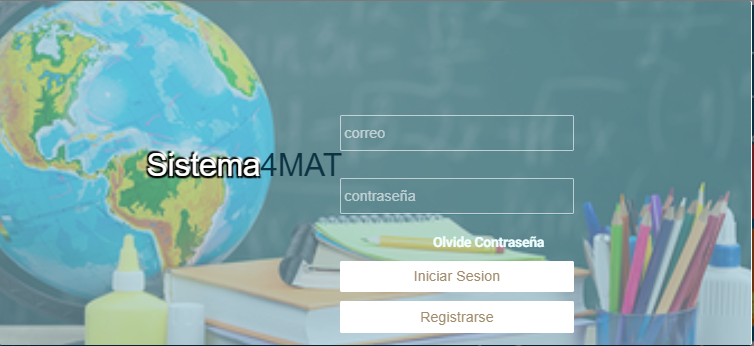
\includegraphics[scale=0.3]{images/Interfaz/IUGS00_login.png}
		\caption{Iniciar sesión}
	\end{figure}

%%\section{Información general de Iniciar sesión}
%%	\subsection{Información del usuario}

\subsection{Información de los préstamos}

\subsection{Información de la encuesta}


\section{Paso 1. Iniciar sesión}
	Se ingresan los datos de identificación para iniciar una sesión.
\subsection{Subpaso 1-A: Ingresar credenciales}
\begin{itemize}
	\item Ingrese identificador.
	\item Ingrese contraseña.
	\item Presione el botón \textbf{Entrar}. Este paso puede derivar
		en los errores \textbf{Error E1-A}, \textbf{Error E1-B} y 
		\textbf{Error E1-C}.
\end{itemize}
Observación 1: un identificador está compuesto por diez dígitos.

\subsection{Error E1-A: usuario no registrado}
El identificador que se ingresó no se encuentra registrado en el sistema,
debe dirigirse al Departamento de Apoyo Técnico para registrarlo.
\begin{itemize}
	\item Presionar \textbf{Aceptar} en la ventana emergente 
		\textbf{IUGS-30: usuario no registrado}
\end{itemize}

\subsection{Error E1-B: contraseña equivocada}
La contraseña que ingresó no concuerda con el valor que se tiene almacenado.
\begin{itemize}
	\item Presionar \textbf{Aceptar} en la ventana emergente 
		\textbf{IUGS-31: contraseña equivocada}
\end{itemize}

\subsection{Error E1-C: solicitante sancionado}
Usted ha sido sancionado por el Departamento de Apoyo Técnico.
\begin{itemize}
	\item Presionar \textbf{Aceptar} en la ventana emergente 
		\textbf{IUGS-32: solicitante sancionado}
\end{itemize}
	\subsection{Bienvenida del administrador de 4MAT}

Se muestra la interfaz de bienvenida.
	\begin{figure}[hbtp]
		\centering
		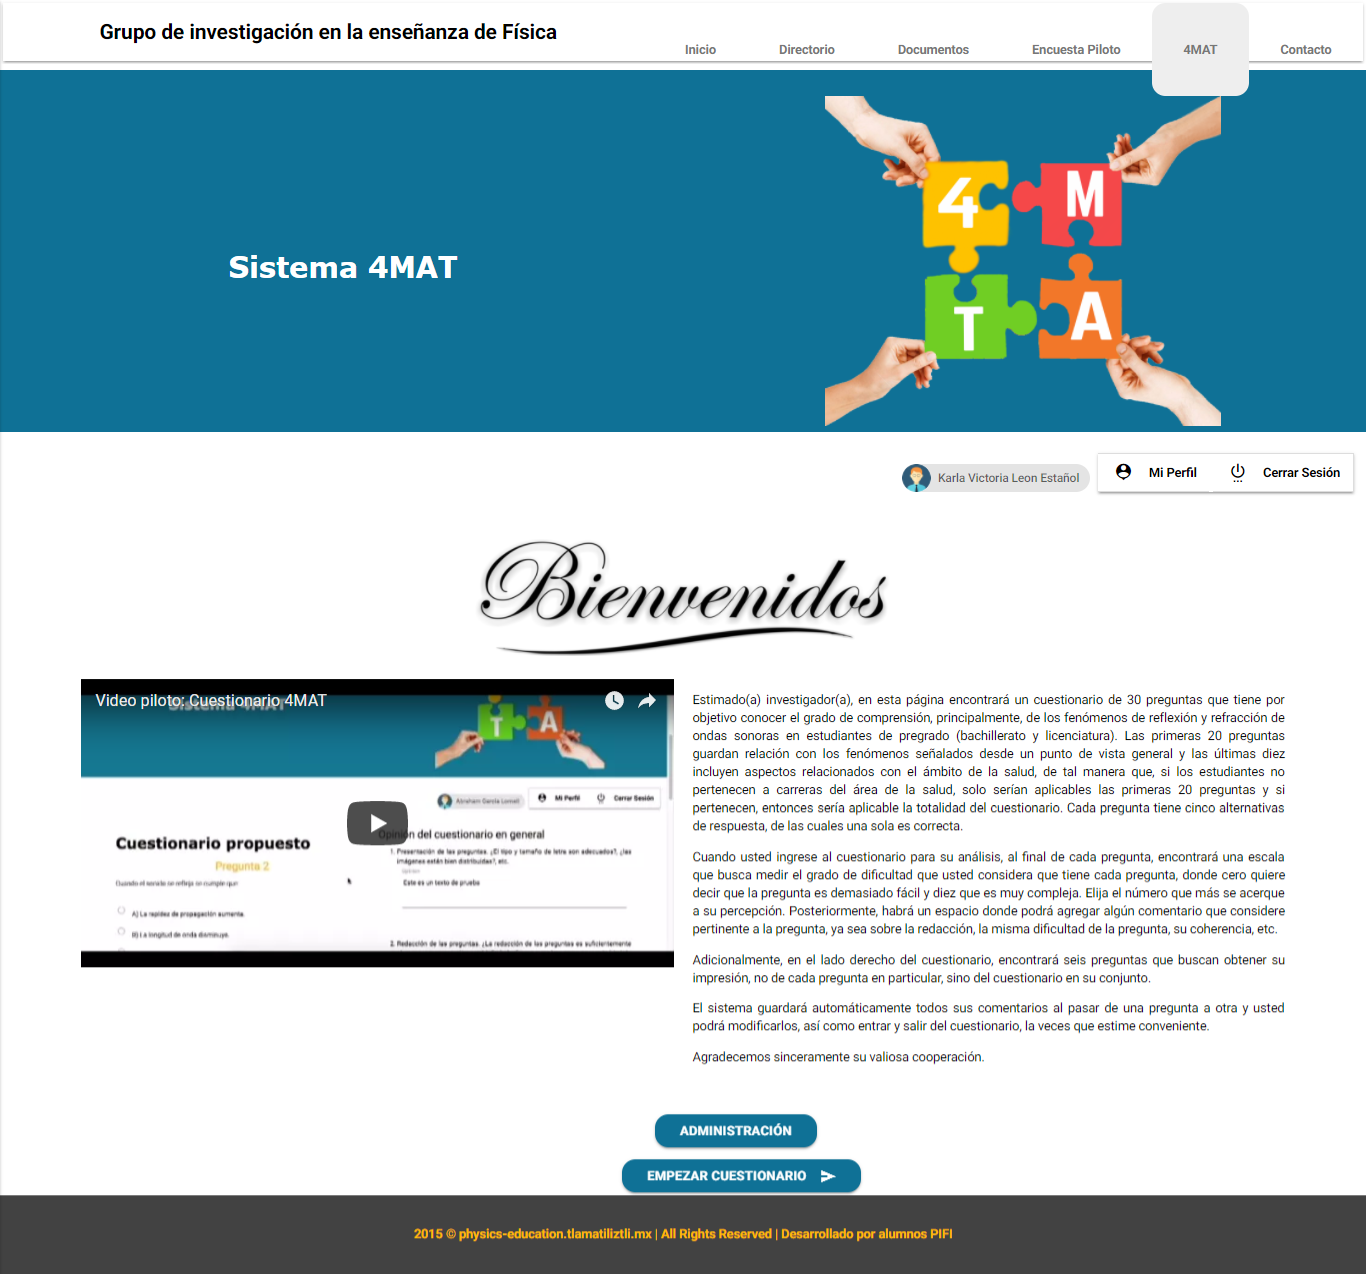
\includegraphics[scale=0.3]{images/Interfaz/IUGS01_binevenida.png}
		\caption{Bienvenida para Administrador}
	\end{figure}
	
La cual contiene los siguientes elementos:
	\begin{itemize}
		\item Menú para las demás secciones de la pagina
			\begin{figure}[hbtp]
		
			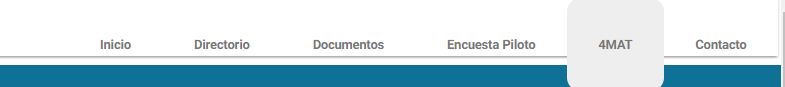
\includegraphics[scale=0.6]{images/Interfaz/IUGS01_menu.png}
			\caption{Menú}
		\end{figure}
		\item Menú de administración de usuario.
			\begin{figure}[hbtp]
		
			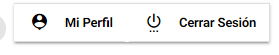
\includegraphics[scale=0.6]{images/Interfaz/IUGS01_menuadmin.png}
			\caption{Menú para datos personales}
		\end{figure}
		
		\item Vídeo explicando como usar la pagina web
		 \begin{figure}[hbtp]
		
			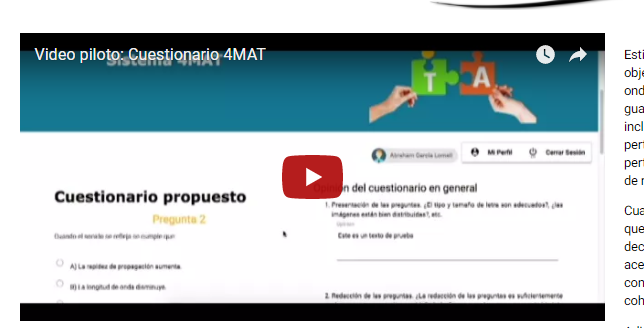
\includegraphics[scale=0.6]{images/Interfaz/IUGS01_video.png}
			\caption{Vídeo explicativo}
		\end{figure}
		\item Botón de administración para consultar estadísticas.
			 \begin{figure}[hbtp]
		
			
\includegraphics[scale=0.6]{images/Interfaz/IUGS01_botonadmin.png}
			\caption{Botón de administración}
		\end{figure}
		\item Botón de iniciar cuestionario. Donde nos presentará el
		cuestionario que se aplicó a los maestros y estudiantes.
		
		
	\end{itemize}
	
	
\chapter{Proceso Reagendar}
	Permite al solicitante cambiar la fecha de asignación de una sala 

\section{Paso 1 de Reagendar}
	El solicitante debe conocer la fecha a la cual se trasladará la nueva
petición

\subsection{Subpaso 1-A: Reagendar}
\begin{enumerate}
	\item De clic al botón  \textbf{Reagendar} mostrado en la interfaz  \textbf{IUGS-02 Reagendar}
\end{enumerate}

	\begin{figure}[hbtp]	
		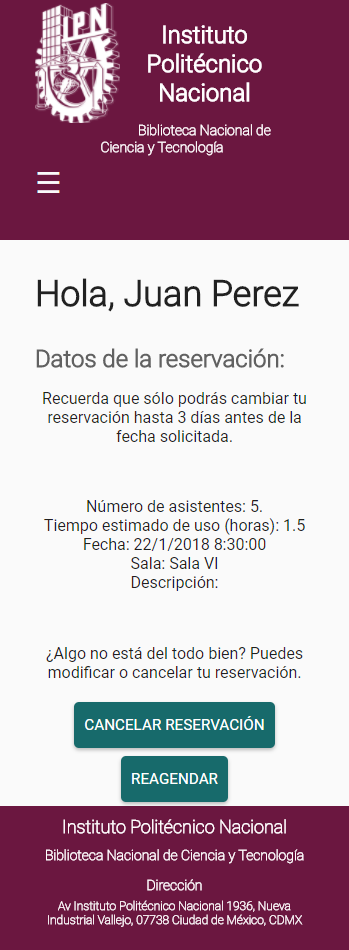
\includegraphics[scale=0.3]{images/InterfazMovil/IUGS05_binevenida.png}
		\caption{Bienvenida para Solicitante}
	\end{figure}
	
\section{Paso 2 de Reagendar}
	\subsection{Subpaso 2-A: Seleccionar día}
\begin{enumerate}
	\item De clic sobre el día deseado mostrado en el calendario de la interfaz  \textbf{IUGS-03 Seleccionar día}
	
\end{enumerate}

	\begin{figure}[hbtp]	
		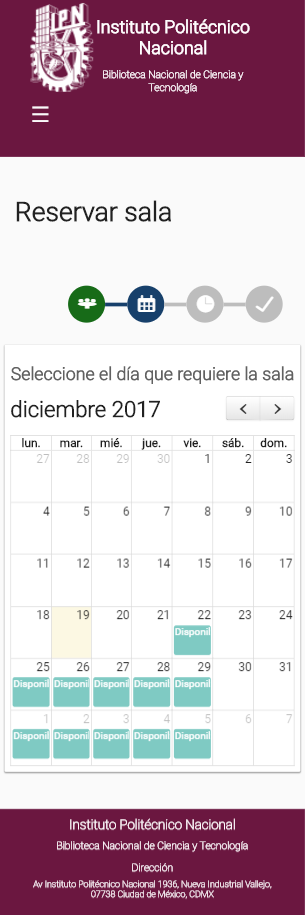
\includegraphics[scale=0.3]{images/InterfazMovil/IUGS02_reservarDiaSolicitante.png}
		\caption{Reservar Día}
	\end{figure}
	
\section{Paso 1 de Reagendar}
	\subsection{Subpaso 3-A: Seleccionar hora}
\begin{enumerate}
	\item Seleccione el intervalo de tiempo deseado (disponible) en la interfaz  \textbf{IUGS-04 Seleccionar hora}
	\item Ingrese la hora inicial.
	\item Ingrese la hora final.
\end{enumerate}
	
\section{Paso 2 de Reagendar}
	\input{PRATS/05_Reagendar/06_confirmación}
	
\chapter{Proceso Reagendar}
	Permite al solicitante cambiar la fecha de asignación de una sala 

\section{Paso 1 de Reagendar}
	El solicitante debe conocer la fecha a la cual se trasladará la nueva
petición

\subsection{Subpaso 1-A: Reagendar}
\begin{enumerate}
	\item De clic al botón  \textbf{Reagendar} mostrado en la interfaz  \textbf{IUGS-02 Reagendar}
\end{enumerate}

	\begin{figure}[hbtp]	
		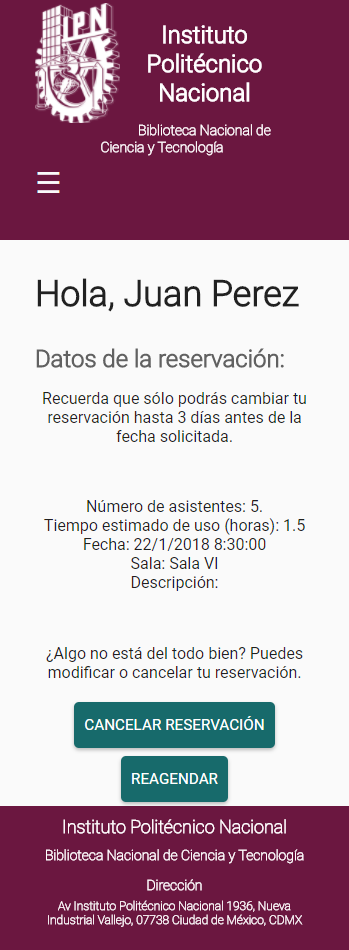
\includegraphics[scale=0.3]{images/InterfazMovil/IUGS05_binevenida.png}
		\caption{Bienvenida para Solicitante}
	\end{figure}
	
\section{Paso 2 de Reagendar}
	\subsection{Subpaso 2-A: Seleccionar día}
\begin{enumerate}
	\item De clic sobre el día deseado mostrado en el calendario de la interfaz  \textbf{IUGS-03 Seleccionar día}
	
\end{enumerate}

	\begin{figure}[hbtp]	
		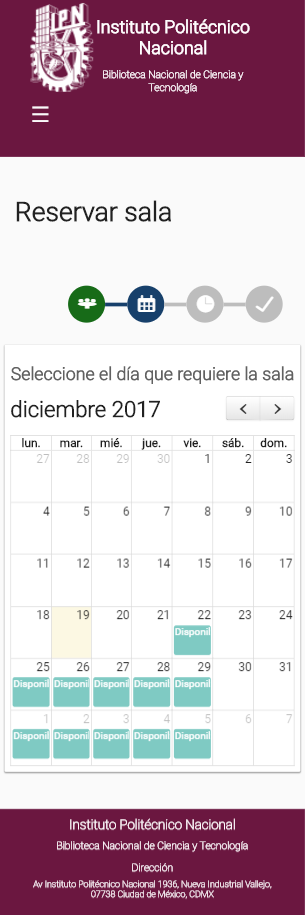
\includegraphics[scale=0.3]{images/InterfazMovil/IUGS02_reservarDiaSolicitante.png}
		\caption{Reservar Día}
	\end{figure}
	
\section{Paso 1 de Reagendar}
	\subsection{Subpaso 3-A: Seleccionar hora}
\begin{enumerate}
	\item Seleccione el intervalo de tiempo deseado (disponible) en la interfaz  \textbf{IUGS-04 Seleccionar hora}
	\item Ingrese la hora inicial.
	\item Ingrese la hora final.
\end{enumerate}
	
\section{Paso 2 de Reagendar}
	\input{PRATS/05_Reagendar/06_confirmación}
	
\chapter{Proceso Reagendar}
	Permite al solicitante cambiar la fecha de asignación de una sala 

\section{Paso 1 de Reagendar}
	El solicitante debe conocer la fecha a la cual se trasladará la nueva
petición

\subsection{Subpaso 1-A: Reagendar}
\begin{enumerate}
	\item De clic al botón  \textbf{Reagendar} mostrado en la interfaz  \textbf{IUGS-02 Reagendar}
\end{enumerate}

	\begin{figure}[hbtp]	
		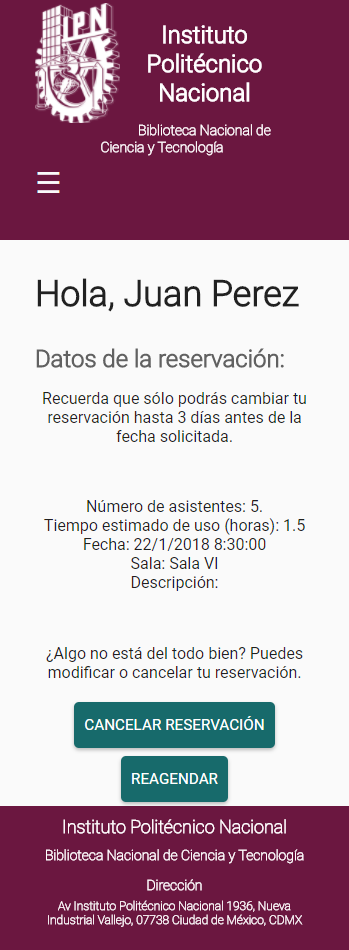
\includegraphics[scale=0.3]{images/InterfazMovil/IUGS05_binevenida.png}
		\caption{Bienvenida para Solicitante}
	\end{figure}
	
\section{Paso 2 de Reagendar}
	\subsection{Subpaso 2-A: Seleccionar día}
\begin{enumerate}
	\item De clic sobre el día deseado mostrado en el calendario de la interfaz  \textbf{IUGS-03 Seleccionar día}
	
\end{enumerate}

	\begin{figure}[hbtp]	
		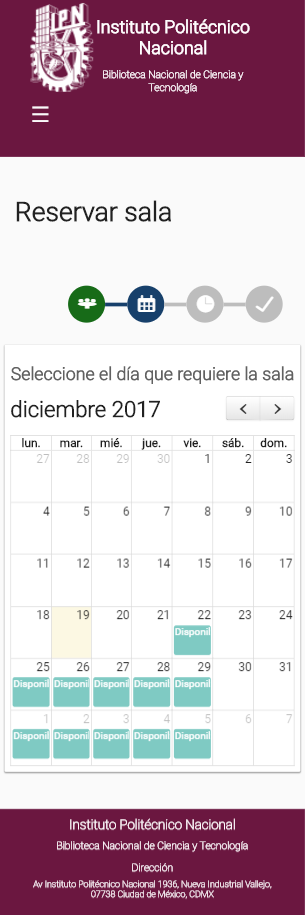
\includegraphics[scale=0.3]{images/InterfazMovil/IUGS02_reservarDiaSolicitante.png}
		\caption{Reservar Día}
	\end{figure}
	
\section{Paso 1 de Reagendar}
	\subsection{Subpaso 3-A: Seleccionar hora}
\begin{enumerate}
	\item Seleccione el intervalo de tiempo deseado (disponible) en la interfaz  \textbf{IUGS-04 Seleccionar hora}
	\item Ingrese la hora inicial.
	\item Ingrese la hora final.
\end{enumerate}
	
\section{Paso 2 de Reagendar}
	\input{PRATS/05_Reagendar/06_confirmación}
	
\chapter{Proceso Reagendar}
	Permite al solicitante cambiar la fecha de asignación de una sala 

\section{Paso 1 de Reagendar}
	El solicitante debe conocer la fecha a la cual se trasladará la nueva
petición

\subsection{Subpaso 1-A: Reagendar}
\begin{enumerate}
	\item De clic al botón  \textbf{Reagendar} mostrado en la interfaz  \textbf{IUGS-02 Reagendar}
\end{enumerate}

	\begin{figure}[hbtp]	
		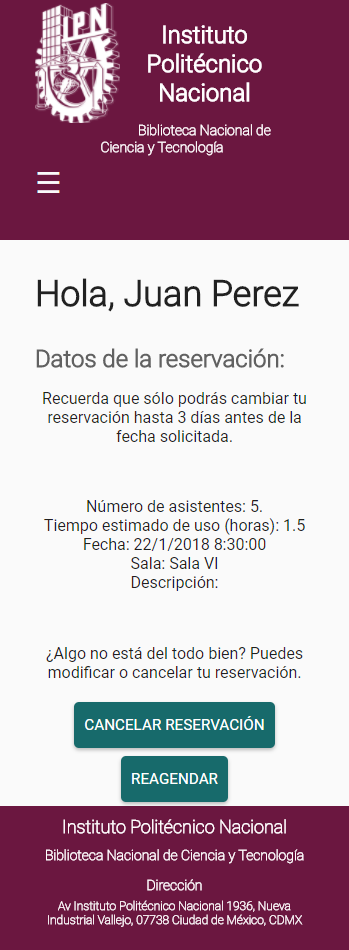
\includegraphics[scale=0.3]{images/InterfazMovil/IUGS05_binevenida.png}
		\caption{Bienvenida para Solicitante}
	\end{figure}
	
\section{Paso 2 de Reagendar}
	\subsection{Subpaso 2-A: Seleccionar día}
\begin{enumerate}
	\item De clic sobre el día deseado mostrado en el calendario de la interfaz  \textbf{IUGS-03 Seleccionar día}
	
\end{enumerate}

	\begin{figure}[hbtp]	
		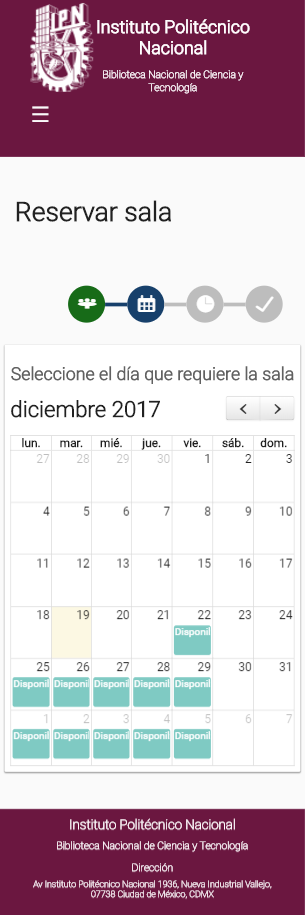
\includegraphics[scale=0.3]{images/InterfazMovil/IUGS02_reservarDiaSolicitante.png}
		\caption{Reservar Día}
	\end{figure}
	
\section{Paso 1 de Reagendar}
	\subsection{Subpaso 3-A: Seleccionar hora}
\begin{enumerate}
	\item Seleccione el intervalo de tiempo deseado (disponible) en la interfaz  \textbf{IUGS-04 Seleccionar hora}
	\item Ingrese la hora inicial.
	\item Ingrese la hora final.
\end{enumerate}
	
\section{Paso 2 de Reagendar}
	\input{PRATS/05_Reagendar/06_confirmación}
	
\chapter{Proceso Reagendar}
	Permite al solicitante cambiar la fecha de asignación de una sala 

\section{Paso 1 de Reagendar}
	El solicitante debe conocer la fecha a la cual se trasladará la nueva
petición

\subsection{Subpaso 1-A: Reagendar}
\begin{enumerate}
	\item De clic al botón  \textbf{Reagendar} mostrado en la interfaz  \textbf{IUGS-02 Reagendar}
\end{enumerate}

	\begin{figure}[hbtp]	
		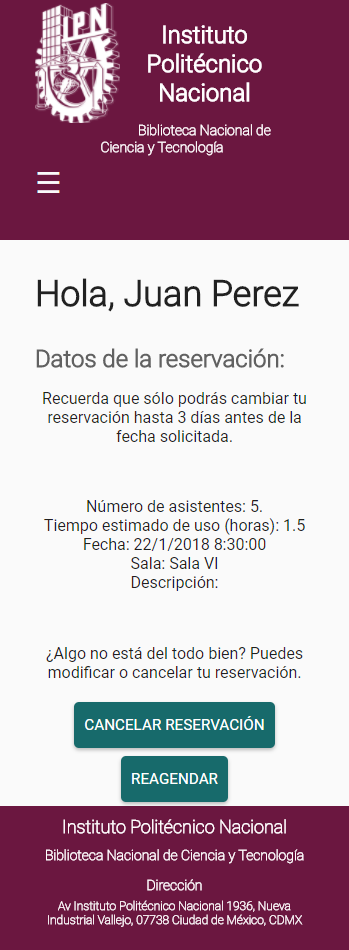
\includegraphics[scale=0.3]{images/InterfazMovil/IUGS05_binevenida.png}
		\caption{Bienvenida para Solicitante}
	\end{figure}
	
\section{Paso 2 de Reagendar}
	\subsection{Subpaso 2-A: Seleccionar día}
\begin{enumerate}
	\item De clic sobre el día deseado mostrado en el calendario de la interfaz  \textbf{IUGS-03 Seleccionar día}
	
\end{enumerate}

	\begin{figure}[hbtp]	
		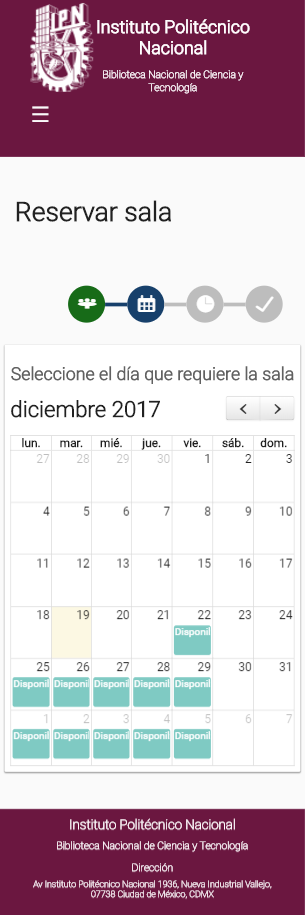
\includegraphics[scale=0.3]{images/InterfazMovil/IUGS02_reservarDiaSolicitante.png}
		\caption{Reservar Día}
	\end{figure}
	
\section{Paso 1 de Reagendar}
	\subsection{Subpaso 3-A: Seleccionar hora}
\begin{enumerate}
	\item Seleccione el intervalo de tiempo deseado (disponible) en la interfaz  \textbf{IUGS-04 Seleccionar hora}
	\item Ingrese la hora inicial.
	\item Ingrese la hora final.
\end{enumerate}
	
\section{Paso 2 de Reagendar}
	\input{PRATS/05_Reagendar/06_confirmación}
	
\chapter{Proceso Reagendar}
	Permite al solicitante cambiar la fecha de asignación de una sala 

\section{Paso 1 de Reagendar}
	El solicitante debe conocer la fecha a la cual se trasladará la nueva
petición

\subsection{Subpaso 1-A: Reagendar}
\begin{enumerate}
	\item De clic al botón  \textbf{Reagendar} mostrado en la interfaz  \textbf{IUGS-02 Reagendar}
\end{enumerate}

	\begin{figure}[hbtp]	
		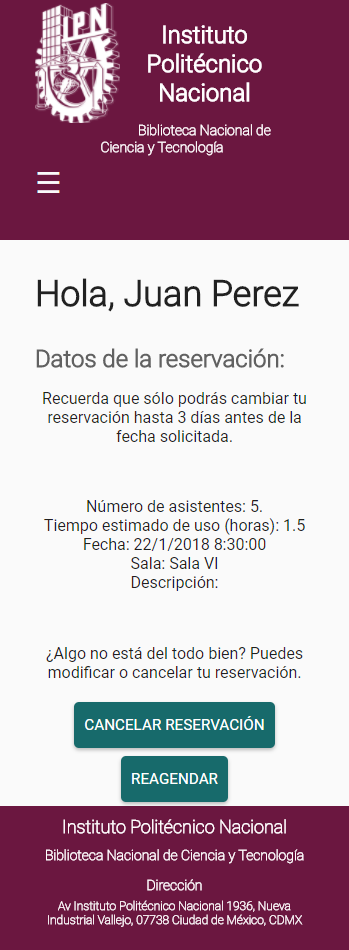
\includegraphics[scale=0.3]{images/InterfazMovil/IUGS05_binevenida.png}
		\caption{Bienvenida para Solicitante}
	\end{figure}
	
\section{Paso 2 de Reagendar}
	\subsection{Subpaso 2-A: Seleccionar día}
\begin{enumerate}
	\item De clic sobre el día deseado mostrado en el calendario de la interfaz  \textbf{IUGS-03 Seleccionar día}
	
\end{enumerate}

	\begin{figure}[hbtp]	
		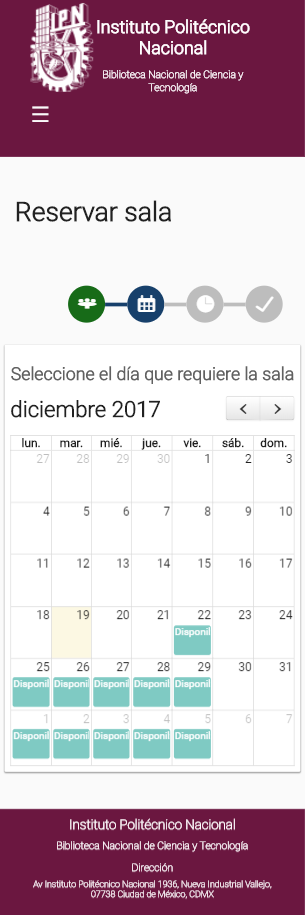
\includegraphics[scale=0.3]{images/InterfazMovil/IUGS02_reservarDiaSolicitante.png}
		\caption{Reservar Día}
	\end{figure}
	
\section{Paso 1 de Reagendar}
	\subsection{Subpaso 3-A: Seleccionar hora}
\begin{enumerate}
	\item Seleccione el intervalo de tiempo deseado (disponible) en la interfaz  \textbf{IUGS-04 Seleccionar hora}
	\item Ingrese la hora inicial.
	\item Ingrese la hora final.
\end{enumerate}
	
\section{Paso 2 de Reagendar}
	\input{PRATS/05_Reagendar/06_confirmación}
	
\chapter{Proceso Reagendar}
	Permite al solicitante cambiar la fecha de asignación de una sala 

\section{Paso 1 de Reagendar}
	El solicitante debe conocer la fecha a la cual se trasladará la nueva
petición

\subsection{Subpaso 1-A: Reagendar}
\begin{enumerate}
	\item De clic al botón  \textbf{Reagendar} mostrado en la interfaz  \textbf{IUGS-02 Reagendar}
\end{enumerate}

	\begin{figure}[hbtp]	
		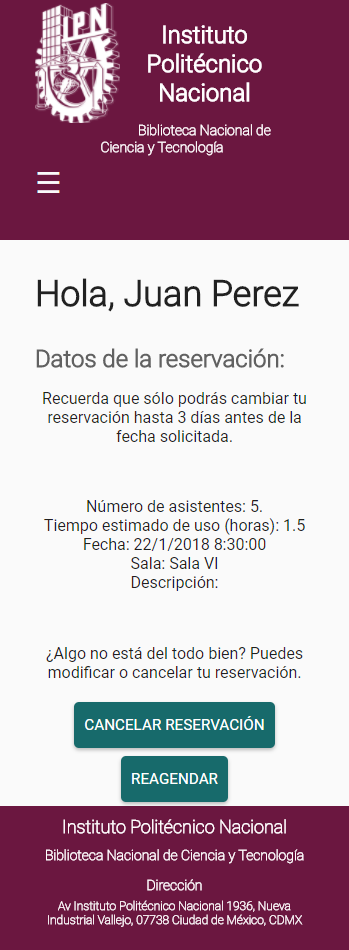
\includegraphics[scale=0.3]{images/InterfazMovil/IUGS05_binevenida.png}
		\caption{Bienvenida para Solicitante}
	\end{figure}
	
\section{Paso 2 de Reagendar}
	\subsection{Subpaso 2-A: Seleccionar día}
\begin{enumerate}
	\item De clic sobre el día deseado mostrado en el calendario de la interfaz  \textbf{IUGS-03 Seleccionar día}
	
\end{enumerate}

	\begin{figure}[hbtp]	
		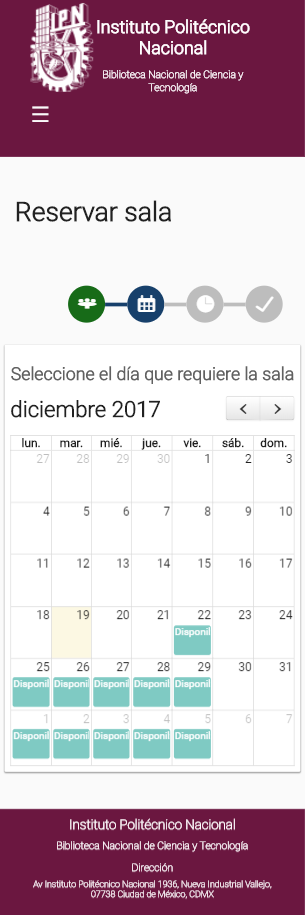
\includegraphics[scale=0.3]{images/InterfazMovil/IUGS02_reservarDiaSolicitante.png}
		\caption{Reservar Día}
	\end{figure}
	
\section{Paso 1 de Reagendar}
	\subsection{Subpaso 3-A: Seleccionar hora}
\begin{enumerate}
	\item Seleccione el intervalo de tiempo deseado (disponible) en la interfaz  \textbf{IUGS-04 Seleccionar hora}
	\item Ingrese la hora inicial.
	\item Ingrese la hora final.
\end{enumerate}
	
\section{Paso 2 de Reagendar}
	\input{PRATS/05_Reagendar/06_confirmación}
	
\chapter{Proceso Reagendar}
	Permite al solicitante cambiar la fecha de asignación de una sala 

\section{Paso 1 de Reagendar}
	El solicitante debe conocer la fecha a la cual se trasladará la nueva
petición

\subsection{Subpaso 1-A: Reagendar}
\begin{enumerate}
	\item De clic al botón  \textbf{Reagendar} mostrado en la interfaz  \textbf{IUGS-02 Reagendar}
\end{enumerate}

	\begin{figure}[hbtp]	
		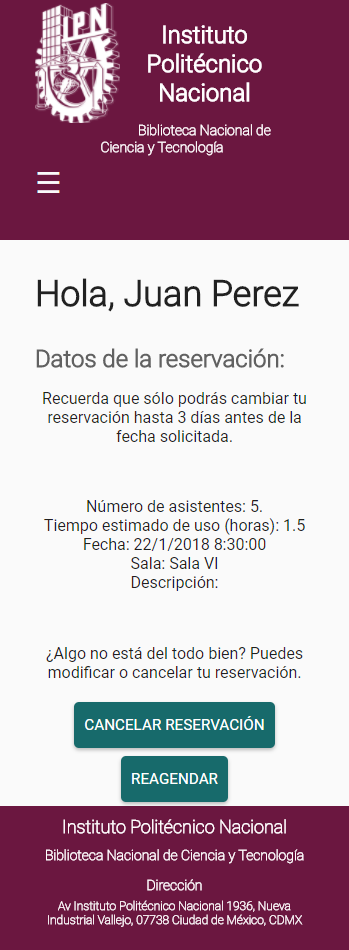
\includegraphics[scale=0.3]{images/InterfazMovil/IUGS05_binevenida.png}
		\caption{Bienvenida para Solicitante}
	\end{figure}
	
\section{Paso 2 de Reagendar}
	\subsection{Subpaso 2-A: Seleccionar día}
\begin{enumerate}
	\item De clic sobre el día deseado mostrado en el calendario de la interfaz  \textbf{IUGS-03 Seleccionar día}
	
\end{enumerate}

	\begin{figure}[hbtp]	
		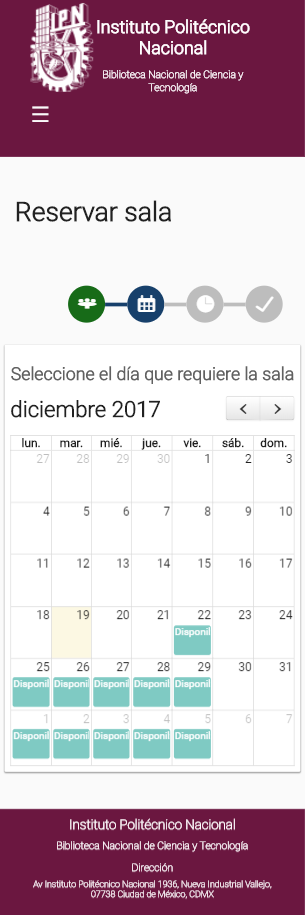
\includegraphics[scale=0.3]{images/InterfazMovil/IUGS02_reservarDiaSolicitante.png}
		\caption{Reservar Día}
	\end{figure}
	
\section{Paso 1 de Reagendar}
	\subsection{Subpaso 3-A: Seleccionar hora}
\begin{enumerate}
	\item Seleccione el intervalo de tiempo deseado (disponible) en la interfaz  \textbf{IUGS-04 Seleccionar hora}
	\item Ingrese la hora inicial.
	\item Ingrese la hora final.
\end{enumerate}
	
\section{Paso 2 de Reagendar}
	\input{PRATS/05_Reagendar/06_confirmación}
	
%% Manual de usuario
%% Departamento de Apoyo Técnico.
%% Índice de los procesos contenidos.

\chapter{Proceso Iniciar Sesión}
	Este capítulo explica el proceso que se lleva a cabo para ingresar al 
	sistema con un identificador y una contraseña. 
	Se tiene la siguiente interfaz:
	
%	\begin{figure}[hbtp]
%		\centering
%		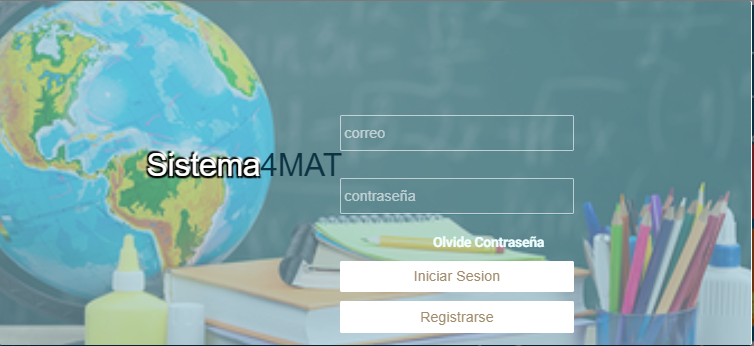
\includegraphics[scale=0.3]{images/Interfaz/IUGS00_login.png}
%		\caption{Iniciar sesión}
%	\end{figure}

%%\section{Información general de Iniciar sesión}
%%	\input{PRATS/01_iniciarSesion/02_informacion}

\section{Paso 1. Iniciar sesión}
	\input{PRATS/01_iniciarSesion/personal/03_iniciarSesion}
	\input{PRATS/01_iniciarSesion/personal/04_bienvenida}
\chapter{Proceso Iniciar Sesión}
	Este capítulo explica el proceso que se lleva a cabo para ingresar al 
	sistema con un identificador y una contraseña. 
	Se tiene la siguiente interfaz:
	
	\begin{figure}[hbtp]
		\centering
		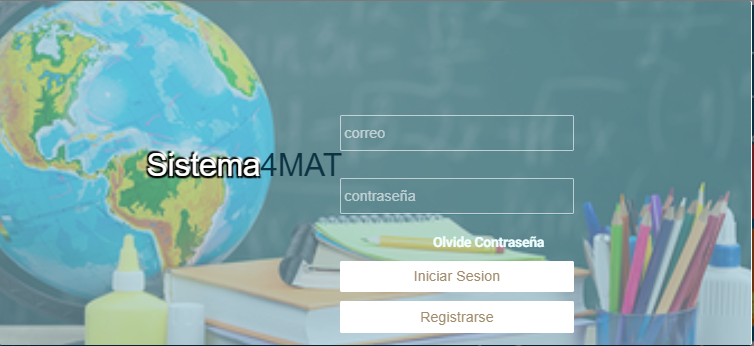
\includegraphics[scale=0.3]{images/Interfaz/IUGS00_login.png}
		\caption{Iniciar sesión}
	\end{figure}

%%\section{Información general de Iniciar sesión}
%%	\input{PRATS/01_iniciarSesion/02_informacion}

\section{Paso 1. Iniciar sesión}
	\input{PRATS/01_iniciarSesion/administrador/03_iniciarSesion}
	\input{PRATS/01_iniciarSesion/administrador/04_bienvenida}
\chapter{Proceso Reagendar}
	Permite al solicitante cambiar la fecha de asignación de una sala 

\section{Paso 1 de Reagendar}
	\input{PRATS/05_Reagendar/03_inicioReag}
	
\section{Paso 2 de Reagendar}
	\input{PRATS/05_Reagendar/04_dia}
	
\section{Paso 1 de Reagendar}
	\input{PRATS/05_Reagendar/05_hora}
	
\section{Paso 2 de Reagendar}
	\input{PRATS/05_Reagendar/06_confirmación}
	
\chapter{Proceso Reagendar}
	Permite al solicitante cambiar la fecha de asignación de una sala 

\section{Paso 1 de Reagendar}
	\input{PRATS/05_Reagendar/03_inicioReag}
	
\section{Paso 2 de Reagendar}
	\input{PRATS/05_Reagendar/04_dia}
	
\section{Paso 1 de Reagendar}
	\input{PRATS/05_Reagendar/05_hora}
	
\section{Paso 2 de Reagendar}
	\input{PRATS/05_Reagendar/06_confirmación}
	
\chapter{Proceso Reagendar}
	Permite al solicitante cambiar la fecha de asignación de una sala 

\section{Paso 1 de Reagendar}
	\input{PRATS/05_Reagendar/03_inicioReag}
	
\section{Paso 2 de Reagendar}
	\input{PRATS/05_Reagendar/04_dia}
	
\section{Paso 1 de Reagendar}
	\input{PRATS/05_Reagendar/05_hora}
	
\section{Paso 2 de Reagendar}
	\input{PRATS/05_Reagendar/06_confirmación}
	
\chapter{Proceso Reagendar}
	Permite al solicitante cambiar la fecha de asignación de una sala 

\section{Paso 1 de Reagendar}
	\input{PRATS/05_Reagendar/03_inicioReag}
	
\section{Paso 2 de Reagendar}
	\input{PRATS/05_Reagendar/04_dia}
	
\section{Paso 1 de Reagendar}
	\input{PRATS/05_Reagendar/05_hora}
	
\section{Paso 2 de Reagendar}
	\input{PRATS/05_Reagendar/06_confirmación}
	
\chapter{Proceso Reagendar}
	Permite al solicitante cambiar la fecha de asignación de una sala 

\section{Paso 1 de Reagendar}
	\input{PRATS/05_Reagendar/03_inicioReag}
	
\section{Paso 2 de Reagendar}
	\input{PRATS/05_Reagendar/04_dia}
	
\section{Paso 1 de Reagendar}
	\input{PRATS/05_Reagendar/05_hora}
	
\section{Paso 2 de Reagendar}
	\input{PRATS/05_Reagendar/06_confirmación}
	
\chapter{Proceso Reagendar}
	Permite al solicitante cambiar la fecha de asignación de una sala 

\section{Paso 1 de Reagendar}
	\input{PRATS/05_Reagendar/03_inicioReag}
	
\section{Paso 2 de Reagendar}
	\input{PRATS/05_Reagendar/04_dia}
	
\section{Paso 1 de Reagendar}
	\input{PRATS/05_Reagendar/05_hora}
	
\section{Paso 2 de Reagendar}
	\input{PRATS/05_Reagendar/06_confirmación}
	
\chapter{Proceso Reagendar}
	Permite al solicitante cambiar la fecha de asignación de una sala 

\section{Paso 1 de Reagendar}
	\input{PRATS/05_Reagendar/03_inicioReag}
	
\section{Paso 2 de Reagendar}
	\input{PRATS/05_Reagendar/04_dia}
	
\section{Paso 1 de Reagendar}
	\input{PRATS/05_Reagendar/05_hora}
	
\section{Paso 2 de Reagendar}
	\input{PRATS/05_Reagendar/06_confirmación}
	
\chapter{Proceso Reagendar}
	Permite al solicitante cambiar la fecha de asignación de una sala 

\section{Paso 1 de Reagendar}
	\input{PRATS/05_Reagendar/03_inicioReag}
	
\section{Paso 2 de Reagendar}
	\input{PRATS/05_Reagendar/04_dia}
	
\section{Paso 1 de Reagendar}
	\input{PRATS/05_Reagendar/05_hora}
	
\section{Paso 2 de Reagendar}
	\input{PRATS/05_Reagendar/06_confirmación}
	
%% Manual de usuario
%% Departamento de Apoyo Técnico.
%% Índice de los procesos contenidos.

\input{PRATS/01_iniciarSesion/01_indicePersonal}
\input{PRATS/06_terminarPrestamo/01_indiceAdministrador}
\input{PRATS/07_sancionarSolcititante/01_indice}
\input{PRATS/08_actualizarUsuario/01_indice}
\input{PRATS/09_BuscarPrestamo/01_indice}
\input{PRATS/11_registrarUsuario/01_indice}
\input{PRATS/10_cerrarSesion/encargado/01_indice}
\input{PRATS/12_extenderPrestamo/01_indice}
\input{PRATS/15_consultarEstadisticas/01_indice}
\input{PRATS/18_cancelarPrestamo/encargado/01_indice}
\input{PRATS/22_buscarUsuario/01_indiceEncargado}
\input{PRATS/14_contestarEncuesta/01_indice}
\input{PRATS/03_registrarPrestamoPresencial/01_indice}

\chapter{Proceso Reagendar}
	Permite al solicitante cambiar la fecha de asignación de una sala 

\section{Paso 1 de Reagendar}
	\input{PRATS/05_Reagendar/03_inicioReag}
	
\section{Paso 2 de Reagendar}
	\input{PRATS/05_Reagendar/04_dia}
	
\section{Paso 1 de Reagendar}
	\input{PRATS/05_Reagendar/05_hora}
	
\section{Paso 2 de Reagendar}
	\input{PRATS/05_Reagendar/06_confirmación}
	
\chapter{Proceso Reagendar}
	Permite al solicitante cambiar la fecha de asignación de una sala 

\section{Paso 1 de Reagendar}
	\input{PRATS/05_Reagendar/03_inicioReag}
	
\section{Paso 2 de Reagendar}
	\input{PRATS/05_Reagendar/04_dia}
	
\section{Paso 1 de Reagendar}
	\input{PRATS/05_Reagendar/05_hora}
	
\section{Paso 2 de Reagendar}
	\input{PRATS/05_Reagendar/06_confirmación}
	

\chapter{Proceso Reagendar}
	Permite al solicitante cambiar la fecha de asignación de una sala 

\section{Paso 1 de Reagendar}
	El solicitante debe conocer la fecha a la cual se trasladará la nueva
petición

\subsection{Subpaso 1-A: Reagendar}
\begin{enumerate}
	\item De clic al botón  \textbf{Reagendar} mostrado en la interfaz  \textbf{IUGS-02 Reagendar}
\end{enumerate}

	\begin{figure}[hbtp]	
		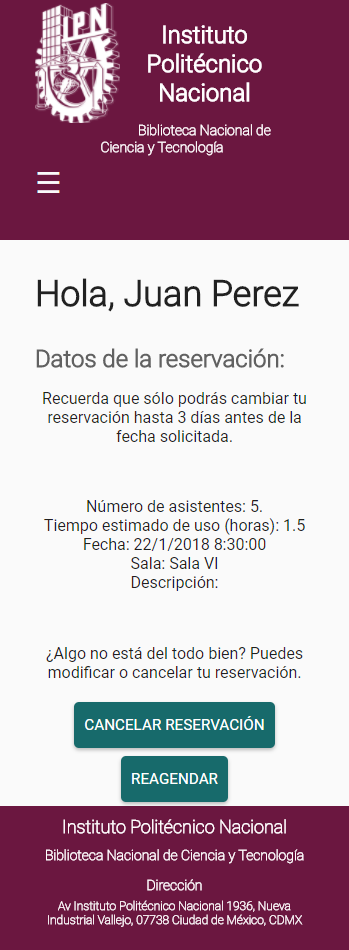
\includegraphics[scale=0.3]{images/InterfazMovil/IUGS05_binevenida.png}
		\caption{Bienvenida para Solicitante}
	\end{figure}
	
\section{Paso 2 de Reagendar}
	\subsection{Subpaso 2-A: Seleccionar día}
\begin{enumerate}
	\item De clic sobre el día deseado mostrado en el calendario de la interfaz  \textbf{IUGS-03 Seleccionar día}
	
\end{enumerate}

	\begin{figure}[hbtp]	
		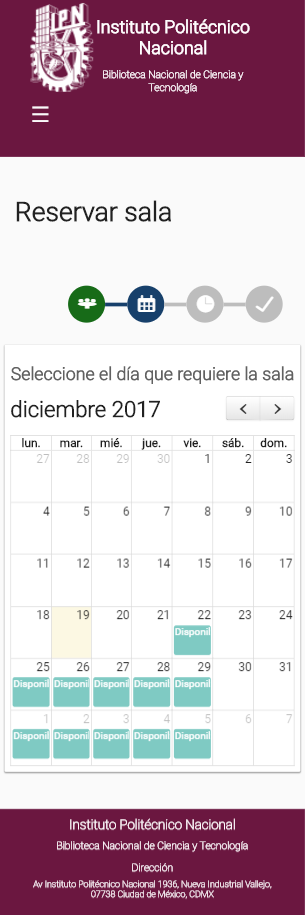
\includegraphics[scale=0.3]{images/InterfazMovil/IUGS02_reservarDiaSolicitante.png}
		\caption{Reservar Día}
	\end{figure}
	
\section{Paso 1 de Reagendar}
	\subsection{Subpaso 3-A: Seleccionar hora}
\begin{enumerate}
	\item Seleccione el intervalo de tiempo deseado (disponible) en la interfaz  \textbf{IUGS-04 Seleccionar hora}
	\item Ingrese la hora inicial.
	\item Ingrese la hora final.
\end{enumerate}
	
\section{Paso 2 de Reagendar}
	\input{PRATS/05_Reagendar/06_confirmación}
	
\chapter{Proceso Reagendar}
	Permite al solicitante cambiar la fecha de asignación de una sala 

\section{Paso 1 de Reagendar}
	El solicitante debe conocer la fecha a la cual se trasladará la nueva
petición

\subsection{Subpaso 1-A: Reagendar}
\begin{enumerate}
	\item De clic al botón  \textbf{Reagendar} mostrado en la interfaz  \textbf{IUGS-02 Reagendar}
\end{enumerate}

	\begin{figure}[hbtp]	
		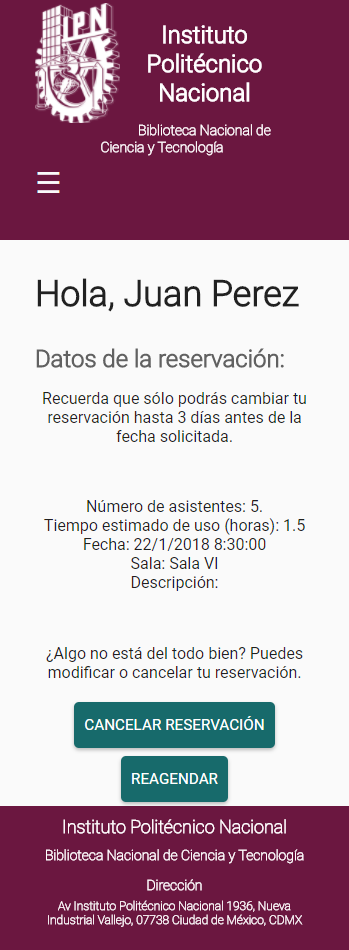
\includegraphics[scale=0.3]{images/InterfazMovil/IUGS05_binevenida.png}
		\caption{Bienvenida para Solicitante}
	\end{figure}
	
\section{Paso 2 de Reagendar}
	\subsection{Subpaso 2-A: Seleccionar día}
\begin{enumerate}
	\item De clic sobre el día deseado mostrado en el calendario de la interfaz  \textbf{IUGS-03 Seleccionar día}
	
\end{enumerate}

	\begin{figure}[hbtp]	
		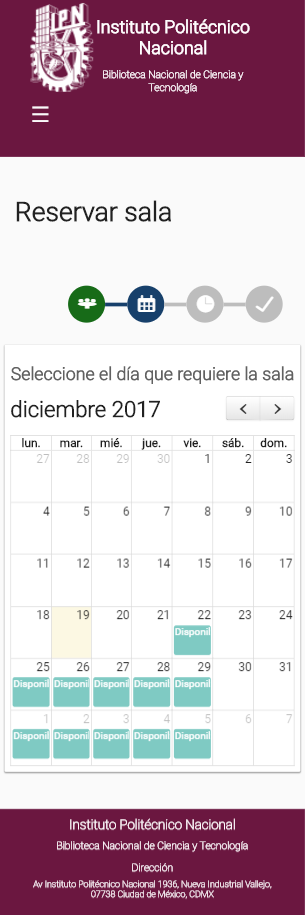
\includegraphics[scale=0.3]{images/InterfazMovil/IUGS02_reservarDiaSolicitante.png}
		\caption{Reservar Día}
	\end{figure}
	
\section{Paso 1 de Reagendar}
	\subsection{Subpaso 3-A: Seleccionar hora}
\begin{enumerate}
	\item Seleccione el intervalo de tiempo deseado (disponible) en la interfaz  \textbf{IUGS-04 Seleccionar hora}
	\item Ingrese la hora inicial.
	\item Ingrese la hora final.
\end{enumerate}
	
\section{Paso 2 de Reagendar}
	\input{PRATS/05_Reagendar/06_confirmación}
	


%%\input{images/interfaces/ApoyoTecnico/pantallas}
\end{document}
